\chapter{WikiMining framework design}
\label{cap:wikimining}

The framework is in an \emph{alpha} development state. While all the described
functionality is implemented and works accordingly, you might sometimes find
yourself needing to change the code in order to tweak some of the behaviour or
that it might not be straight-forward to extend the framework with some
specific complex functionality. However, I intend to bring it to a quality
standard that will allow you to perform both of the above tasks with ease.

\section{External libraries}

As part of the WikiMining we use multiple external libraries that we quickly
describe in the following subsections.

\subsection{Java Wikipedia Library}

\ac{JWPL} is an open-source library that facilitates access to a lot of
information concerning Wikipedia including, but not limited to:
\begin{itemize}
  \item page link graph
  \item category link graph
  \item page \(\leftrightarrow\) category link graph
  \item page content (MediaWiki and plain-text formats)
\end{itemize}

\paragraph{How it works?} Given a Wikipedia dump - that can be downloaded from
\url{http://dumps.wikimedia.org/} (accessed on 17.04.2014)i - it
generates \(11\) text files that can then be imported into a MySQL databased
and accessed through the \ac{JWPL} \ac{API}.
You can find more details about using \ac{JWPL} on their website
\footnote{\url{https://code.google.com/p/jwpl/wiki/DataMachine} (accessed on
17.04.2014) }.

The library is publicly available
\footnote{\url{https://code.google.com/p/jwpl/} (accessed on 17.04.2014)} and
its authors wrote a paper \cite{zesch2008jwpl} providing further insights into
how it works. For the purposes of this thesis we use \emph{\ac{JWPL} 0.9.2}.

\subsection{Hadoop}

\emph{Hadoop} is an open-source project that aims to offer solutions for
'reliable, scalable, distributed computing'
\footnote{\url{http://hadoop.apache.org/} - accessed on 17.04.2014)}.  Although
the whole system is more complex we mainly use two of its components:
\begin{itemize}
  \item \acl{MR}
  \item \acl{HDFS}
\end{itemize}

\subsubsection{MapReduce}

\acf{MR} is a two-phase process that borrows two concepts from functional
programming:
\begin{itemize}
  \item map;
  \item reduce;
\end{itemize}
and applies them to distributed computing.
The main steps are as follows:
\begin{enumerate}
  \item In the first stage - the map stage - the data is partitioned and spread
  across multiple processes that perform the same task and output multiple
  (key, value) pairs.
  \item In-between the two phases, the results from the first stage are
  collected and sorted by key in a distributed fashion.
  \item In the second stage - the reduce stage - all pairs that share the same
  key are sent to the same process and this task outputs a results based on the
  received pairs (that share the same key).
\end{enumerate}
\acf{MR} is a very powerful technique for doing distributed computations
because it provides an easy way to write distributed code that is both
fault-tolerant and free from other distributed computing problems (such as
synchronisation concerns, deadlocks etc.).
If you are interested in learning more about \acf{MR} we recommend reading the
paper \cite{dean2008mapreduce} written by its proponents.

\subsubsection{Hadoop Distributed File System}

\acf{HDFS} is, as it name says, a distributed file-system that offers the
file-system back-end for writing \acl{MR} jobs and using other Hadoop-based
frameworks. Its purpose is to store large-scale data reliably and
distributively such that it can be easy to stream this data at a high bandwidth
to applications running on multiple machines \cite{shvachko2010hadoop}.

For the purposes of this thesis we use \emph{Hadoop 1.0.4} and \emph{Hadoop
2.2.0} for \cloud.

\subsection{\cloud}

\emph{\cloud} is an open source library for processing \emph{big data} that
runs over \emph{Hadoop 2}. \cloud provides the following features:
\begin{itemize}
  \item frequently used Hadoop data types;
  \item basic graph algorithms: bread-first search, PageRank;
  \item a Wikipedia \ac{API}.
\end{itemize}
In this thesis we use the Wikipedia \ac{API} to convert the \ac{XML} dumps to
Hadoop \emph{sequence files} indexed by \emph{document id}. This allows us to
easily find specific Wikipedia pages and process their content.

If you want to find out more about \cloud, visit their website
\footnote{\url{http://lintool.github.io/cloud} (accessed on 17.04.2014)} or
check their Wikipedia \ac{API}
\footnote{\url{http://lintool.github.io/cloud/docs/content/wikipedia.html}
(accessed on 17.04.2014)}. In this thesis we use \emph{\cloud version 1.5.0}.

\subsection{Mahout}

\emph{Mahout} is a scalable machine learning library designed to run over very
large data sets using Hadoop \acl{MR}. While it offers distributed algorithms
for a lot of machine learning problems such as:
\begin{itemize}
  \item classification
  \item clustering
  \item recommendations
\end{itemize}
we are only using Mahout for indexing Wikipedia and creating the corresponding
tf-idf vectors.

\paragraph{Generating tf-idf vectors} To create tf-idf vectors from a set of
plain-text documents \footnote{Stored in a \ac{HDFS}-specific format called
Sequence Files.} is being done using \emph{mahout seq2sparse}. This tool has
parameters that allow us to filter out rare words, stop-words and even perform
stemming if needed.

If you are interested in finding out more about Mahout you can read the book
\emph{Mahout in Action} \cite{owen2011mahout} or visit their website
\footnote{\url{https://mahout.apache.org/} (accessed on 17.04.2014)}. For the
purposes of this thesis we use \emph{Mahout version 0.9}.

\section{System architecture}
\label{sec:arch}

In this section, we describe how we designed and implemented the WikiMining
library for summarising Wikipedia using submodular function maximisation.
In Figure~\ref{fig:wikimining} we present the general architecture of
WikiMining.

\begin{figure}
  \centering
  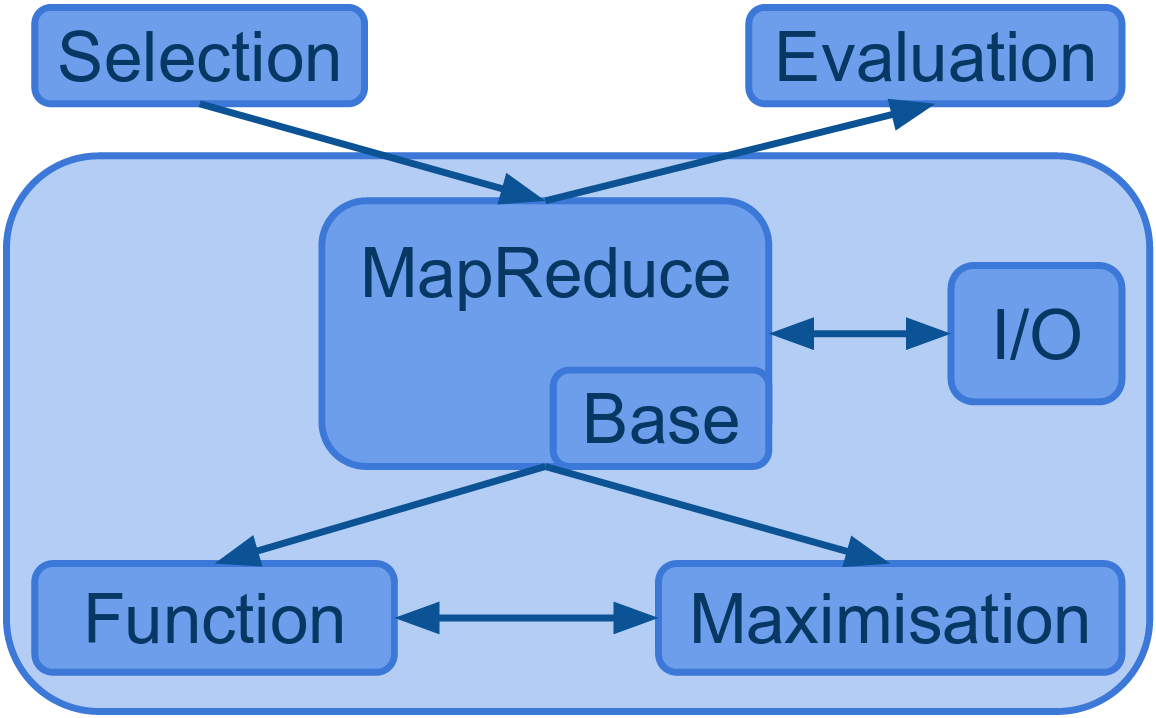
\includegraphics[width=0.5\textwidth,natwidth=1156,natheight=718]{images/wikimining.png}
  \caption{WikiMining architecture overview.}
  \label{fig:wikimining}
\end{figure}

\subsection{Base data types}

We use the following data type classes, defined in package
\emph{ch.ethz.las.wikimining.base}:
\begin{description}
  \item[ArrayWritable] Different subclasses for serialiasing an array of
  different types:
    \begin{itemize}
      \item \emph{IntArrayWritable} - for integers: \emph{IntWritable};
      \item \emph{TextArrayWritable} - for strings: \emph{Text};
    \end{itemize}
  or offer more functionality such as print its content in plain text using a
  \emph{toString()} method.
  \item[DocumentWithVector] An (Integer document id, Vector) pair used in a lot
  of MapReduces to partition the data as part of:
    \begin{itemize}
      \item the GreeDi protocol (see Section~\vref{sec:submod-max});
      \item \acl{LSH} (see Section~\vref{sec:lsh}).
    \end{itemize}
    It also comes in a \emph{Writable} form so that it can be serialisable by
    Hadoop \acl{MR}.
  \item[HashBandWritable] A (hash, band) pair used for \ac{LSH}.
  \item[SquaredNearestNeighbour] A collection that gets the nearest neighbour
  of an article (based on cosine similarity) from among the documents that were
  written before the input article. This is used to compute \emph{document
  influence}.
  \item[Vector] Class from Mahout that represents a \emph{double}-valued
  mathematical vector. It comes in two flavours:
  \begin{itemize}
    \item \emph{DenseVector} - stored as a normal array
    \item \emph{RandomAccessSparseVector} - stored as a hash-map of indexes to
    values.
  \end{itemize}
\end{description}

In addition we have two classes for:
\begin{itemize}
  \item storing the default parameters - \emph{Defaults}
  \item defining the program arguments - \emph{Fields}
\end{itemize}

\subsection{Submodular functions}

Given that the \emph{GreeDi} protocol has only general, high-level restrictions
(such as being able to partition the data for example), we can easily implement
submodular functions similarly to implementing them in other programming
language. Also the \emph{submodular function maximisation} algorithms are
implemented such that they can correctly work with any submodular function that
extends the \emph{ObjectiveFunction} interface - which is very non-restrictive.

WikiMining provides the following submodular functions package
\emph{ch.ethz.las.wikimining.functions}:
\begin{description}
  \item[CombinerWordCoverage] Implements the function described in
  Section~\vref{sec:word-coverage++}, whose \emph{coverage of a word} function
  uses \emph{tf-idf}, \emph{number of inlinks}, \emph{number of revisions} and
  \emph{revision volume}.
  \item[CutFunction] Given a graph split, it compute the maximum cut value. It
  is not used with Wikipedia, but instead we used it to test our implementation
  correctness against the \emph{SFO Matlab toolbox} \cite{krause2010sfo}.
  \item[DocumentInfluence] Computes the \emph{influence of a document} as
  described in Section~\vref{sec:doc-influence} and
  Section~\vref{sec:scale-doc-influence}, given the \emph{document creation
  dates}, a \emph{document novelty} index and a \emph{yearly word spread}
  index.
  \item[GraphCoverage] Computes the \emph{graph coverage} described in
  Section~\vref{sec:graph-coverage}, given the graph as an \emph{adjacency
  list}.
  \item[LSHBuckets] Computes the \emph{\ac{LSH}-buckets} function described in
  Section~\vref{sec:lsh-buckets}, given the \ac{LSH} buckets.
  \item[ObjectiveCombiner] Linearly combines multiple objective functions as
  described in Section~\vref{sec:combine}, given a list of
  functions and weights.
  \item[RevisionsSummer] A \emph{modular} function that just sums the number of
  revisions of each selected document.
  \item[WeightedWordCoverage] Implements the \emph{word coverage} function
  where:
    \begin{itemize}
      \item \emph{word importance} is defined as in
      Section~\vref{sec:word-coverage++};
      \item \emph{coverage of a word} uses just the \emph{tf-idf} as described
      in Section~\vref{sec:word-coverage};
    \end{itemize}
  \item[WordCoverageFromMahout] Implements the same \emph{word coverage}
  function as above (WeightedWordCoverage), except that it ignores the
  \emph{word importance}, considered to be a \emph{constant \(1\)}.
\end{description}
All functions that need the \emph{tf-idf} vectors expect them as a
\emph{HashMap} from \emph{document ids} to \emph{Mahout Vectors}.

If you are interested in implementing your own submodular functions, you just
need to implement the \emph{ObjectiveFunction} interface such that your class
provides a \emph{compute} method which returns the \emph{double} score of a set
of \emph{document ids}.

\subsection{Submodular function maximisation}

WikiMining provides three types of greedy \acf{SFO} algorithms in package
\emph{ch.ethz.las.wikimining.sfo}:
\begin{description}
  \item[SfoGreedyLazy] Implements a lazy greedy \ac{SFO} algorithm that uses a
  non-stable sorting mechanism, that is a heap, to speed-up the computations as
  described in Section~\vref{sec:submod-functions}. This is the only
  maximisation algorithm that we use in all our non-testing code. It has a
  complexity of \(O(k \cdot avgN\), where \(k\) is the number of selected
  documents and \(avgN\) is the average number times the current top value of
  the heap is not the real maximum score.
  \item[SfoGreedyNonLazy] Implements a brute-force (non-lazy) - it tries all
  possible documents at each iteration - greedy \ac{SFO} algorithm as described
  in Section~\vref{sec:submod-functions}.
  \item[SfoGreedyStableLazy] Implements a stable-sort lazy greedy \ac{SFO}
  algorithm. The complexity of this algorithm is the same as of the non-lazy
  version: \(O(k \cdot N)\), where \(k\) is the desired number of selected
  documents and \(N\) is the total number of documents; as a results, it isn't
  really useful, but we used it for testing and debugging.
\end{description}

If you need to implement your own \acl{SFO} algorithm you would need to
implement the \emph{SfoGreedyAlgorithm} interface such that your class provides
the two synonymous \emph{run} methods which take a \emph{list of ids} and the
\emph{number of elements to select} and return the \emph{selected document
ids}. Instead, if you are interested in using more of our already implemented
code and structure you can consider extending the \emph{AbstractSfoGreedy}
abstract class that provides you with \emph{score, document id} pair.

\subsection{Coverage \aclp{MR}}

This part refers to the three categories of classes that deal with coverage,
found in package \emph{ch.ethz.las.wikimining.mr.coverage[.h104]}:
\begin{enumerate}
  \item preprocessing classes;
  \item GreeDi protocol classes;
  \item reducer classes.
\end{enumerate}

The preprocessing classes are as follows:
\begin{description}
  \item[GraphEdgesConvertor] Converts a plain-text \emph{list of edges} to an
  \emph{adjacency list} saved in a sequence file.
  \item[GraphInlinksCounter] Given the inverted adjacency lists it computes the
  number of inlinks of each node.
  \item[RevisionsConvertor] Converts a list of \emph{revision statistics}
  (number of revisions, revision volume from plain-text to sequence files;
  \item[WikiToPlainText] Converts an \ac{XML} Wikipedia dump to plain-text
  sequence files, using \cloud.
\end{description}

The two stages of the \emph{GreeDi} protocol are implemented as classes
\emph{GreeDiFirst} and \emph{GreeDiSecond}. These two classes are very similar
in implementation and they deal with:
\begin{itemize}
  \item parsing the program arguments;
  \item reading the main input files - the tf-idf vectors;
  \item setting up the desired reducer.
\end{itemize}
They also include the \emph{mapper} implementations which are simple as their
only job is to partition the data.

While the \emph{mappers} for the GreeDi protocol are simple and are almost
always the same, independent of the used submodular functions being used, the
\emph{reducers} have to deal with reading all the additional data for the more
complex submodular functions (for example, the graph, the revision statistics).
We implement the following reducers:
\begin{description}
  \item[CombinerGreeDiReducer] Read multiple statistics - such as word count,
  LSH-buckets, graph, revisions - and uses submodular functions that combines
  them together \footnote{See Section~\vref{sec:word-coverage++}};
  \item[CoverageGreeDiReducer] Reads as less as possible to apply either the
  simple word coverage with a \emph{word importance} of \(1\) or with
  \emph{word importance} as word count or document count \footnote{See
  Section~\vref{sec:word-coverage++}};
  \item[GraphGreeDiReducer] Reads the graph and applies \emph{graph coverage}
  by itself \footnote{See Section~\vref{sec:graph-coverage}};
  \item[LshBucketsGreeDiReducer] Reads the \ac{LSH} buckets and applies the
  \emph{\ac{LSH} buckets function}. \footnote{See
  Section~\vref{sec:lsh-buckets}}.
\end{description}

\subsection{Influence \aclp{MR}}

The influence classes, from package
\emph{ch.ethz.las.wikimining.mr.influence[.h104]}, can also be split in the same
three categories as the coverage classes:
\begin{enumerate}
  \item preprocessing classes;
  \item GreeDi protocol classes;
  \item reducer classes.
\end{enumerate}

The preprocessing classes are as follows:
\begin{description}
  \item[DocumentDate] Given Wikipedia's \ac{XML} dump it retrieves the last
  modified date of each article;
  \item[GenerateBasisMatrix] Generates the (bands, rows) random projections
  matrix needed for the cosine-similarity \ac{LSH};
  \item[TfidfNovelty] Computes the \emph{document novelty score} \footnote{See
  Section~\vref{sec:doc-influence} and Section~\vref{sec:scale-doc-influence}};
  \item[TfIdfRemoveDuplicates] Removes duplicates (possibly) generated by
    \emph{TfIdfNovelty};
  \item[TfIdfWordSpread] Computes the yearly \emph{word spread} \footnote{See
    Section~\vref{sec:doc-influence}};
\end{description}

The two stages of the \emph{GreeDi} protocol are implemented as classes
\emph{GreeDiFirst} and \emph{GreeDiSecond} and are very similar to their
\emph{coverage} counterparts discussed above.

We implement the following reducers:
\begin{description}
  \item[GreeDiReducer] Applies the \ac{SFO} greedy algorithm for influential
  documents as a Reduce stage, part of the GreeDi protocol;
  \item[TfIdfNoveltyReducer] Used by \emph{TfIdfNovelty} to compute the
  documents \ac{kNN} and then use them to compute the document \emph{novelty}
  score;
  \item[TfIdfNoveltyIdentityReducer] Outputs the buckets themselves so that we
  can use them as part of other objective functions.
\end{description}

\subsection{Selection and evaluation}

Classes from  package \emph{ch.ethz.las.wikimining.evaluate} deal with
selecting single or multiple Wikipedia categories and offer basic capabilities
to analyze the results.

The most important classes of this package are:
\begin{description}
  \item[WikiRandomSelect] Given the tf-idf vectors file -- needed to get the
  document ids -- randomly samples (with replacement) a given number of
  Wikipedia articles;
  \item[WikiExtractor] Given the categories names as arguments it extracts the
  requested categories and saves them in sequence file format;
  \item[WikiCountInlinks] Converts a list of articles ids into a list of
  (article name, number of inlinks) pairs, using \ac{JWPL}.
\end{description}

\subsection{Input, output}

Classes from package \emph{ch.ethz.las.wikimining.mr.io.h104} simplify the way
one can deal with Hadoop \ac{IO}.
It offers \textbf{SetupHelper} class to easily set the desired input and output
format for Hadoop and a lot of \emph{SequenceFileProcessor} classes to read
(and write) different \emph{sequence file}.
Some examples include:
\begin{description}
  \item[BucketsSequenceFileReader] Reads (HashBandWritable, IntArrayWritable)
  pairs, used for the \emph{\ac{LSH} buckets} function \footnote{See
  Section~\vref{sec:lsh-buckets}};
  \item[IntLongSequenceFileReader] Reads (IntWritable, LongWritable) pairs,
  used in multiple classes;
  \item[TextVectorSequenceFileReader] Reads (Text, VectorWritable) pairs, used
  in multiple classes to read the \emph{tf-idf vectors};
  \item[TextVectorSequenceFileWriter] Writes (Text, VectorWritable) pairs, used
  to output the \emph{novelty vectors} \footnote{See Section~\vref{sec:doc-influence} and Section~\vref{sec:scale-doc-influence}}.
\end{description}

